%%%%%%%%%%%%%%%%%%%%%%%%%%%%%%%%%%%%%%%%%%%%%%%%
% 4: Diseño y resolución del trabajo realizado
%%%%%%%%%%%%%%%%%%%%%%%%%%%%%%%%%%%%%%%%%%%%%%%%
\chapter{Diseño y resolución del trabajo realizado}
\label{diseno}

Después de estudiar cual es la situación actual de la enseñanza de la programación a un nivel global y los diferentes proyectos que promueven el \emph{pensamiento computacional}, en este capítulo se analizarán cuales son las necesidades del proyecto Robode y como se han resuelto.

Como ya se ha mencionado anteriormente, se creará un simulador de un robot, al que hemos denominado \emph{Robode}, y se integrará en la plataforma Descubre la programación. Robode  estará dentro de un mundo del que podrá moverse con libertad y con el que podrá interactuar. El robot tendrá dos ruedas que se mueven independientemente (con un motor para cada una de ellas) y dispondrá de sensores que informarán de posibles colisiones con el robot. También, el robot tendrá la capacidad de detectar lineas o caminos pintados en el suelo, sabiendo también en que dirección detecta (o no) la linea.

Adicionalmente, el robot y el mundo en el que este se encuentra será dibujado en un elemento \emph{canvas} de HTML5, al igual que ocurre en la plataforma Descubre.


Como se puede ver, Robode es la unión de varios de los proyectos que se han analizado en el capítulo \ref{estado-arte}. Por una parte, la idea principal de crear un simulador es igual a la que se ha realizado en Robomind (el cual se analiza en la sección \ref{sec:robomind}) pero simulando un robot en un mundo continuo y con características similares a las de Moway (analizado en la sección \ref{sec:moway}). Por último, se ejecutará en un entorno web, como bien puede ser el ejemplo de las herramientas que proporcionan CodeHS (sección \ref{sec:CodeHS}) y Code.org (sección \ref{sec:Code.org}). 


En las secciones siguientes se va a estudiar como se ha diseñado y creado Robode, que características tiene y cual ha sido la implementación exacta llevada a cabo.



\section{Motor de físicas}
\label{sec:mundo}


Para la creación del mundo y de las físicas que gestionan las colisiones y la interacción entre todos los elementos del simulador se ha optado por entre dos librerías físicas: PhysicsJS\footnote{Página oficial de la librería PhysicsJS (\url{http://wellcaffeinated.net/PhysicsJS}).} y Box2d \cite{box2d. Dos librerías de software libre y que trabajan sobre entornos web, más en concreto Javascript.

Ambas librerías son muy versátiles pero PhysicsJS tiene está aún en fase beta y, por otra parte, Box2D tiene una gran comunidad de programadores utilizando dicha librería, lo cual siempre es de ayuda para resolver dudas y solucionar problemas.

Por tanto, se ha elegido la librería Box2D para implementar el simulador de Robode. En realidad, Box2D es una famosa librería implementada originalmente para Flash\footnote{Página oficial de la librería Box2D para Flash (\url{http://www.box2dflash.org}).} que ha sido portada a Javascript dos veces. Una de ellas por Yayushi Ando y se llama Box2Djs\footnote{Página oficial de Box2Djs (\url{http://box2d-js.sourceforge.net}).}. El otro intento de llevar Box2D a Javascript ha culminado en Box2Dweb\footnote{El repositorio de Box2Dweb está alojado en GitHub (\url{https://github.com/hecht-software/box2dweb}).}. Al final se ha escogido Box2Dweb, puesto que tiene una gran comunidad utilizando dicha librería y, en cambio, Box2Djs está desactualizada y es necesario realizar importaciones de muchos ficheros en cada proyecto, al contrario que pasa con Box2Dweb.

Una vez que se ha aclarado que la librería utilizada es \texttt{Box2Dweb}, por simplicidad, a partir de ahora nos referiremos a ésta simplemente como \texttt{Box2D}.

\subsection{Definición del Mundo}

\texttt{Box2D} tiene una serie de elementos básicos que afectan al diseño y uso de nuestro simulador. Estos son: el Mundo (World), los Cuerpos (Bodies), los Accesorios (Fixtures) y las Articulaciones o elementos constrictores (Joints).

El núcleo del motor de físicas en \texttt{Box2D} es el Mundo (\emph{World}). \emph{World} define los parámetros básicos que regirán la simulación más tarde, como puede ser el ratio de actualización o la gravedad. También contiene y controla el resto de elementos: \emph{Bodies}, \emph{Fixtures} y \emph{Joints} entre otros.



Para la creación de nuestro mundo, hemos decidido que tendrá una vista \emph{top-down}, es decir, una vista del mundo desde arriba, desde el cielo. De esta manera se consigue una vista superior de todo el circuito simplificando la comprensión del movimiento del robot sobre el circuito.

Una de las características más importantes de \texttt{Box2D} es la posibilidad de dotar a la aplicación que se está creando de un efecto gravitatorio de manera nativa al motor. Lo normal sería establecer éste valor con un vector de dirección hacia el suelo (hacia la parte baja de la pantalla) con la fuerza que se quiera simular. Esto provocaría que los cuerpos del mundo estuvieran constantemente sometidos a una fuerza que los mueve en dirección a ese vector, normalmente hacia el suelo.  

En el caso de Robode, al tener una vista superior del circuito, establecer una gravedad provocaría que el robot y el resto de cuerpos del circuito se movieran de forma anómala. Por esto, es necesario crear un mundo sin gravedad. En el código \ref{code:world-gravedad} podemos ver como se ha establecido la gravedad del mundo a un vector con valor 0 en ambos ejes de coordenadas. 

\begin{lstlisting}[language={Javascript},label={code:world-gravedad}, caption={Definición del objeto \texttt{World} en Box2D con gravedad 0 y permitiendo que los cuerpos sean capaces de dormir.}]
Simulator.World = new b2World(
	new b2Vec2(0, 0), //gravity
	true //allow sleep
);
\end{lstlisting}

Otra característica importante en Box2D y que tiene un gran impacto en el rendimiento de la simulación es que los cuerpos puedan \emph{dormir}. Un cuerpo \emph{dormirá} cuando éste esté inactivo, es decir, cuando no esté siendo sometido a ninguna fuerza o sobre el se aplican fuerzas, pero éstas no son capaces de alterar su estado (posición, ángulo de giro, etc)\footnote{Esto ocurre generalmente cuando un objeto está sobre una superficie cuya forma y la del cuerpo hace que éste se mantenga quieto. Un ejemplo de esto puede ser un cuadrado sobre una superficie plana y horizontal con una gravedad hacia el suelo.}. En la linea 3 del código \ref{code:world-gravedad} se puede ver como se ha establecido que los cuerpos del mundo sean capaces de dormir. Así, se consigue que el motor no simule los cuerpos que estén inactivos, mejorando el rendimiento de la aplicación.

Por último, queda definir el \emph{paso del tiempo} en Box2D. Para ello, es necesario ejecutar la función \texttt{Simulator.World.Step()} cada vez que queramos que se ejecute un \emph{paso} en nuestro mundo (esto es equivalente a un \emph{tic} de reloj). Esta función ordenará al motor que aplique todas las fuerzas necesarias sobre los cuerpos del mundo (gravedad, colisiones, deslizamientos, etc). Obviamente, es en este momento cuando se ejecutará la detección de colisiones por parte del motor de físicas. Justo después de ejecutar un paso se deben eliminar las fuerzas que afectan a los objetos para que se produzca un movimiento y efecto natural de las distintas fuerzas en los cuerpos. Esto se consigue con la función \texttt{Simulator.World.ClearForces()}.

En el código \ref{code:world-step} se puede ver con más detalle las funciones básicas que se deben ejecutar para que se produzca una actualización del mundo en Box2D.

\begin{lstlisting}[language={Javascript},label={code:world-step}, caption={Actualización del mundo en \texttt{Box2D}.}]
// (...)
Simulator.World.Step(
	1 / 60, //frame-rate
	10, //velocity iterations
	10 //position iterations
);

Simulator.World.ClearForces();

// (...)
\end{lstlisting}


\subsubsection{Creación de elementos en Box2D}


La creación de elementos (\emph{bodies}, \emph{fixtures}, \emph{joints}, etc) en Box2D utiliza un \emph{patrón factoría}, teniendo que definir primero en un objeto plantilla (definición) las características que tendrá el elemento a crear.

En el código \ref{code:ejemplo-factoria} se puede ver como se crea el cuerpo principal del robot utilizando una factoría tanto para definir el objeto \emph{Body} como la \emph{Fixture} a partir de \emph{World}, que realizará la creación del mismo.

\begin{lstlisting}[language={Javascript},label={code:ejemplo-factoria}, caption={Creación del cuerpo principal del robot utilizando la librería Box2dweb.}]
// Body definition
var bodyDef = new b2BodyDef(); 
bodyDef.type = b2Body.b2_dynamicBody;
bodyDef.position.Set(posX, posY);
bodyDef.linearDamping = 8;
bodyDef.angularDamping = 8;

// Fixture definition
var fixDef = new b2FixtureDef(); 
fixDef.density = 40;
fixDef.friction = 1;
fixDef.restitution = 0;
// Polygon Shape as a box
fixDef.shape = new b2PolygonShape(); 
fixDef.shape.SetAsBox(width, height);

// Create BODY robot
var robot = Simulator.World.CreateBody(bodyDef);
robot.setName("robot");

// Add fixture to body
robot.CreateFixture(fixDef);
\end{lstlisting}


El elemento \emph{Body} será el que contenga la información básica del objeto, como es su posición, velocidad o ángulo de giro. Será el elemento \emph{Fixture} el que defina la forma (si es un polígono o círculo y de que forma) y sus características (fricción que produce, densidad, etc) del \emph{Body} al que está asociado.


\subsection{Construcción del robot}
\label{sec:contruccion-robot}


Anteriormente ya se ha mencionado que el robot tendrá 2 ruedas, 2 sensores que detectarán lineas y otros 4 que detectaran colisiones. El cuerpo del robot será modelado con un rectángulo, cuyo ancho es menor que el largo. Las dos ruedas se dispondrán en cada lado del cuerpo principal, un poco retrasadas de la mitad del cuerpo.

Los 4 sensores de colisión serán modelados con triángulos y estarán dispuestos de forma que sobresalgan del cuerpo principal con la base del triángulo hacía el exterior, para así poder detectar colisiones antes de que ocurran. Las posiciones de cada uno de los 4 sensores se han descrito con las posiciones cardinales: noroeste, sureste, noreste y sureste. 

De esta manera, el robot tendrá 2 sensores que detectan colisiones en la parte delantera y otros dos en la trasera. 

Los sensores que detectan lineas serán modelados como círculos simulando dos cámaras mirando al suelo, igual que ocurre en el robot Moway. 

Todos estos elementos del robot están modelados en cuerpos separados. No obstante, es necesario que se mantengan unidos y se muevan a la vez. Es aquí donde entran en juego los \emph{joints}. Usaremos un joint de tipo \texttt{Revolute}, que permite definir una unión entre dos cuerpos como si fuera una cuerda de tamaño fijo, manteniendo la distancia por la que se separan ambos cuerpos. Por tanto, tendremos 8 joints que unen el cuerpo principal con las partes del robot (2 ruedas, 2 sensores de linea y 4 sensores de colisión.).
 
El código Javascript que crea el robot ya se ha visto en el código \ref{ejemplo-factoria}. Los valores de densidad, fricción y restitución\footnote{La restitución de un cuerpo es la capacidad que tiene el mismo de \emph{rebotar} contra una superficie contra la que choca. Por ejemplo, una pelota cayendo sobre una superficie plana rebotará con una fuerza igual a la velocidad con la que ha golpeado la superficie si el valor es 1. Con valor 0, se desactiva esta propiedad.} serán 40, 1 y 0, respectivamente. Estos valores se mantendrán iguales en todos los cuerpos creados, para dar una sensación de uniformidad en las colisiones. Cuanto mayor sea la densidad de un cuerpo, mayor será su masa. Los valores de fricción y restitución van de 0 a 1, siendo 0 un valor que anula la propiedad. 
 
 
En la figura \ref{fig:robot-skel} se puede ver el esqueleto del robot con todos los elementos juntos. 

\begin{figure}[!ht]
	\begin{centering}
		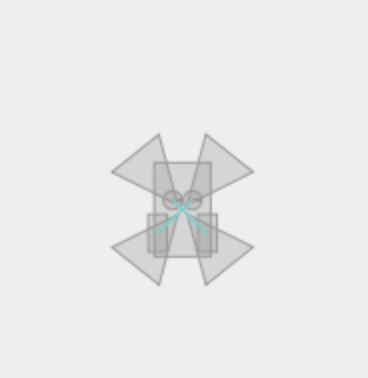
\includegraphics[width=0.5\textwidth]{images/robot-skel.png}
			\caption{Esqueleto del robot que muestra los diferentes \emph{bodies} y \emph{joints} que lo forman.}
				\label{fig:robot-skel}
	\end{centering}
\end{figure}


\subsubsection{Ruedas}

La característica principal de un \texttt{Revolute Joint} es la posibilidad de establecer  un límite para que los cuerpos puedan rotar en función de las anclas que se establecen en cada cuerpo. Así, se puede establecer un motor que simule entre otros ruedas, cadenas o puertas giratorias. Justo lo que se pretende.

El movimiento de las ruedas del robot se simulará con el giro que permite hacer el joint y la velocidad de giro determinará la velocidad a la que se mueve la rueda. En el código \ref{code:wheel-joint} se puede ver la creación de un del joint que une el coche con la rueda.

\begin{lstlisting}[language={Java},label={code:wheel-joint}, caption={Función que crea el joint que une la rueda al coche.}]
function addWheelJoint(mybody, mywheel) {

	var revoluteJointDef = new b2RevoluteJointDef();
	revoluteJointDef.Initialize(mybody, mywheel, mywheel.GetWorldCenter());

	revoluteJointDef.enableMotor = true;
	revoluteJointDef.motorSpeed = 0;
	revoluteJointDef.maxMotorTorque = Number.MAX_SAFE_INTEGER;
	revoluteJointDef.enableLimit = true;

	return Simulator.World.CreateJoint(revoluteJointDef);
}
\end{lstlisting}

La función \texttt{Initialize()} recibe como parámetros los dos cuerpos que van a ser unidos por el joint y el punto en el que se realizará el ancla (para eso se utilizará la función \texttt{GetWorldCenter()} de la clase \texttt{Body} para obtener el punto del mundo en el que se encuentra un cuerpo).

Se activará la propiedad de motor en las ruedas y se le dará un valor inicial de 0. También se establecerá el valor máximo de torsión del joint para evitar que ante una fuerza de giro muy grande, el joint se mueva de su sitio. Por último, se activará un límite para que las ruedas no se muevan de su sitio ya que es esta propiedad la que define si el ancla será fija o permitirá movimiento con respecto a la separación de los dos cuerpos.


\subsubsection*{Sensores}
{\color{green} ===POR AQUI===}.


\subsection{Moviendo a Robode}
\label{moviendo-robode}

%velocidad de las ruedas, cancelación velocidad lateral, movimiento...
% hablar propiedades de los cuerpos y fixtures 


\subsection{Detectando colisiones}
\label{detectando-colisiones}



\subsection{Detectando lineas}
\label{detectando-lineas}

\subsubsection{Curvas de Bezier}
\label{bezier}

%Uno de los aspectos más importantes en Robode es la capacidad del mismo de poder detectar lineas. La finalidad de esto es que se pueda programar un comportamiento \emph{sigue-lineas}. Para ello, era necesario responder a una serie de preguntas:
%\begin{enumerate}
%	\item ¿Cómo se representan las lineas pintadas en el suelo?
%	\item ¿Cómo se modelan dichas lineas?
%\end{enumerate}


\subsection{Animando a Robode}
\label{animando-robode}

%\subsubsection{Multihilo y esas cosas}
Aquí se habla de como se anima y que tiene que decir JS y su sistema monohilo al respecto. También temas de zoom y scroll



\subsection{Construcción de circuitos}
\label{sec:construccion-circuitos}



%El entorno o circuito por el que se moverá el robot tiene los siguientes elementos: (a) obstáculos, con los que podrá chocar y que se desplazaran por la colisión; (b) fronteras, que no podrán ser desplazadas o atravesadas por el robot y (c) lineas, que no producirán una colisión pero que podrán ser detectadas por el robot. 



\section{Integración en Descubre}
\label{sec:integracion-descubre}

\subsection{Modificación del lenguaje iJava}
\label{sec:modificacion-ijava}


